\documentclass[11pt,a4paper]{article}
\usepackage[utf8]{inputenc}
\usepackage{color,graphicx}
\usepackage{amsmath}
\usepackage{amssymb}
\usepackage{tikz}
\usetikzlibrary{decorations.markings,arrows.meta}
\usepackage{pgfplots}
\usepgfplotslibrary{colormaps}
\usepackage{tcolorbox}  
\usetikzlibrary{hobby}
\usetikzlibrary {arrows.meta}
\usepackage{xcolor}
\pgfplotsset{compat=1.18}

\begin{document}

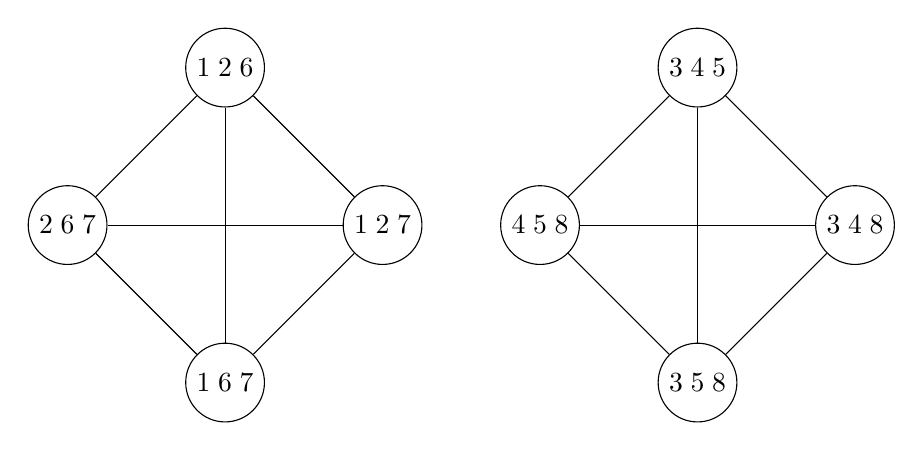
\begin{tikzpicture}[
  % diamond-friendly node style
  vertex/.style={circle,draw=black,minimum size=10mm,inner sep=0pt},
  line/.style={draw=black}
]

\node[vertex] (A) at (0, 2) {$1 \; 2 \; 6$};  % top
\node[vertex] (B) at (2, 0) {$1 \; 2 \; 7$};  % right
\node[vertex] (C) at (0,-2) {$1 \; 6 \; 7$};  % bottom
\node[vertex] (D) at (-2,0) {$2 \; 6 \; 7$};  % left

% edges (K4) — explicit
\draw[line] (A)--(B);
\draw[line] (A)--(C);
\draw[line] (A)--(D);
\draw[line] (B)--(C);
\draw[line] (B)--(D);
\draw[line] (C)--(D);

\node[vertex] (E) at (6, 2) {$3 \; 4 \; 5$};  % top
\node[vertex] (F) at (8, 0) {$3 \; 4 \; 8$};  % right
\node[vertex] (G) at (6,-2) {$3 \; 5 \; 8$};  % bottom
\node[vertex] (H) at (4, 0) {$4 \; 5 \; 8$};  % left

% edges (K4) — explicit
\draw[line] (E)--(F);
\draw[line] (E)--(G);
\draw[line] (E)--(H);
\draw[line] (F)--(G);
\draw[line] (F)--(H);
\draw[line] (G)--(H);

\end{tikzpicture}

\end{document}